\documentclass[10pt]{article}

\usepackage{amsmath}% amsmath package, useful for mathematical formulas
\usepackage{amssymb}% amssymb package, useful for mathematical symbols
\usepackage{graphicx}
\usepackage{cite}% cite package, to clean up citations in the main text. Do not remove.
\usepackage{color} 
\usepackage[labelfont=bf,labelsep=period,justification=raggedright]{caption}

% Text layout
\topmargin 0.0cm
\oddsidemargin 0.5cm
\evensidemargin 0.5cm
\textwidth 16cm 
\textheight 21cm

\newcommand{\card}[1]{{\lVert#1\rVert}_0}
\newcommand{\mb}{\mathbf}
\newcommand{\norm}[1]{\lVert#1\rVert}
\newcommand\argmin{\operatornamewithlimits{arg\,min}}
\newcommand\argmax{\operatornamewithlimits{arg\,max}}

\author{Amir Kosrowshahi, Urs K\"oster}
\title{Convolutional Sparse Coding}
 
\begin{document}
\maketitle

\section{Sparse coding model}
\label{sec:sparsealg}

Sparse coding~\cite{Olshausen96,olshausen2003learning,Smith:2006qf} is
a latent variable model that attempts to describe data in terms of a
small number of additive components, or basis functions, selected out
of a large dictionary. Let $y_i(t)$, the data on channel $i$ at time
$t$, be written as a temporal convolution of a set of basis functions
$\phi_{ij}(t)$, with $i$ and $j$ denoting channel and basis function,
respectively,
\begin{align}
y_i(t) = \sum_j \phi_{ij}(t) * x_j(t) + \epsilon_{i}(t) \label{eqn:conv}
\end{align}
with $\epsilon_i(t) \sim \mathcal{N}(0,\sigma_n)$ small, uncorrelated
gaussian noise on each channel. This model is illustrated in
Fig.~\ref{fig:sparseconvolution}. To estimate model parameters, the
data is assumed to be an identically distributed, independent ensemble
of length $T$ time samples with $C$ channels $\mb{Y} =
\{\mb{y}^{(i)}\}_{i=1\ldots D}$ with $\mb{y}^{(i)} \in \mathbb{R}^{C
  \times T}$. The log-likelihood of the model is,
\begin{align*}
\mathcal{L}(\mb{\Phi}, \sigma_n)
&= \log p(\mb{Y} | \mb{\Phi}, \sigma_n, \lambda) \\
&= \sum_{i=1}^D \log p(\mb{y}^{(i)} | \mb{\Phi}, \sigma_n, \lambda) \\
&= \sum_{i=1}^D \log \int \mathrm{d} \mb{x} \, p(\mb{y}^{(i)}
| \mb{x}, \mb{\Phi}, \sigma_n) \, p(\mb{x} | \lambda)
\end{align*}
where,
\begin{align*}
  p(\mb{y} | \mb{x}, \mb{\Phi}, \sigma_n) \propto
  \exp\left(-\frac{1}{2 \sigma_n^2} \sum_{t=1}^T \norm{\mb{y}_t -
      \sum_\tau \mb{\Phi}_\tau \mb{x}_{t-\tau}}^2\right)
\end{align*}
with $\mb{\Phi}_\tau \in \mathbb{R}^{C \times N}$, $\mb{x}_\tau \in
\mathbb{R}^N$ with $N$ the number of basis functions. The sparse prior
on the coefficients $\mb{x}$ is parametrized with $\lambda$. The goal
of learning is to maximize the likelihood $\mathcal{L}(\mb{\Phi},
\sigma_n)$. The derivative of $\mathcal{L}(\mb{\Phi}, \sigma_n)$ is
taken with respect to the model parameter $\mathbf{\Phi}_\alpha$,
\begin{align*}
  \frac{\partial \mathcal{L}}{\partial \mathbf{\Phi}_\alpha} &\propto
  - \sum_{i=1}^D {\int \mathrm{d} \mb{x} \, p(\mb{x} | \mb{y}^{(i)},
    \mb{\Phi}, \sigma_n, \lambda) \sum_{t=1}^T (\mb{y}_t - \sum_\tau
    \mb{\Phi}_\tau \mb{x}_{t-\tau}) \,\mb{x}_{t-\alpha}^T}
\end{align*}
A number of ways exist to estimate the intractable integral in this
expression, including a Laplace
approximation~\cite{lewicki1999probabilistic} and Hamiltonian Monte
Carlo sampling~\cite{culpepperbuilding}. The simplest approach, taken
here, is to assume the posterior distribution $p(\mb{x} |
\mb{y}^{(i)}, \mb{\Phi}, \sigma_n, \lambda)$ is sufficiently peaked
and to take one sample at its mode~\cite{Olshausen97}, that is,
\begin{align}
  \mb{x}^{(i)} &= \argmax_{\mathbf{x}} p(\mb{x} | \mb{y}^{(i)},
  \mb{\Phi}, \sigma_n,
  \lambda) \nonumber \\
  &= \argmax_{\mb{x}} \log p(\mb{y}^{(i)}, \mb{x} |\mb{\Phi},
  \sigma_n, \lambda) \nonumber \\
  &= \argmin_{\mb{x}}\left( \frac{1}{2 \sigma_n^2} \sum_{t=1}^T
    \norm{\mb{y}_t - \sum_\tau \mb{\Phi}_\tau \mb{x}_{t-\tau}}^2 -
    \log p(\mb{x}|\lambda) \right)\label{eqn:inference}
\end{align}
Model likelihood was maximized using an alternating scheme where
$\mb{x}^{(i)}$ were inferred and then used to update
$\mathcal{L}(\mb{\Phi},\sigma_n)$~\cite{Olshausen97}. An additional
simplifying assumption was made to take the parameter of the gaussian
noise $\sigma_n$ as given, though a prior could be imposed on it and
estimated along with $\mb{\Phi}$. In practice, an appropriate
$\sigma_n$ is approximated from descriptive statistics of the data. As
the data is practically infinite, only a small sample of
$\mb{y}^{(i)}$ was chosen in each step. Additionally, the model has a
degeneracy due to the sparse prior $p(\mb{x}|\lambda)$ shrinking
coefficients to zero, causing the norm of $\mb{\Phi}$ to grow without
bound. Therefore a convex constraint was imposed such that,
\begin{align*}
  \sum_{i=1}^C\sum_{\tau=1}^P\phi_{ij\tau}^2 \le 1
\end{align*}
where $P$ are the number of time taps in the basis functions. The
constraint makes the learning update of $\mb{\Phi}$ a quadratically
constrained quadratic program (QCQP)~\cite{boyd2004convex}. In
practice, however, this problem was solved by making a small
stochastic gradient learning step and renormalizing the basis
functions on each iteration. A full QCQP solver was implemented using
a convolutional adaptation of the method proposed in
\cite{mairal2010online}, but found that for neural datasets, the
algorithm was prone to get stuck in local minima. During learning, the
basis functions were recentered gradually over many iterations. This
reflected an implicit prior that the basis functions should be
temporally localized.

\begin{figure}[ht!]
  \centering
  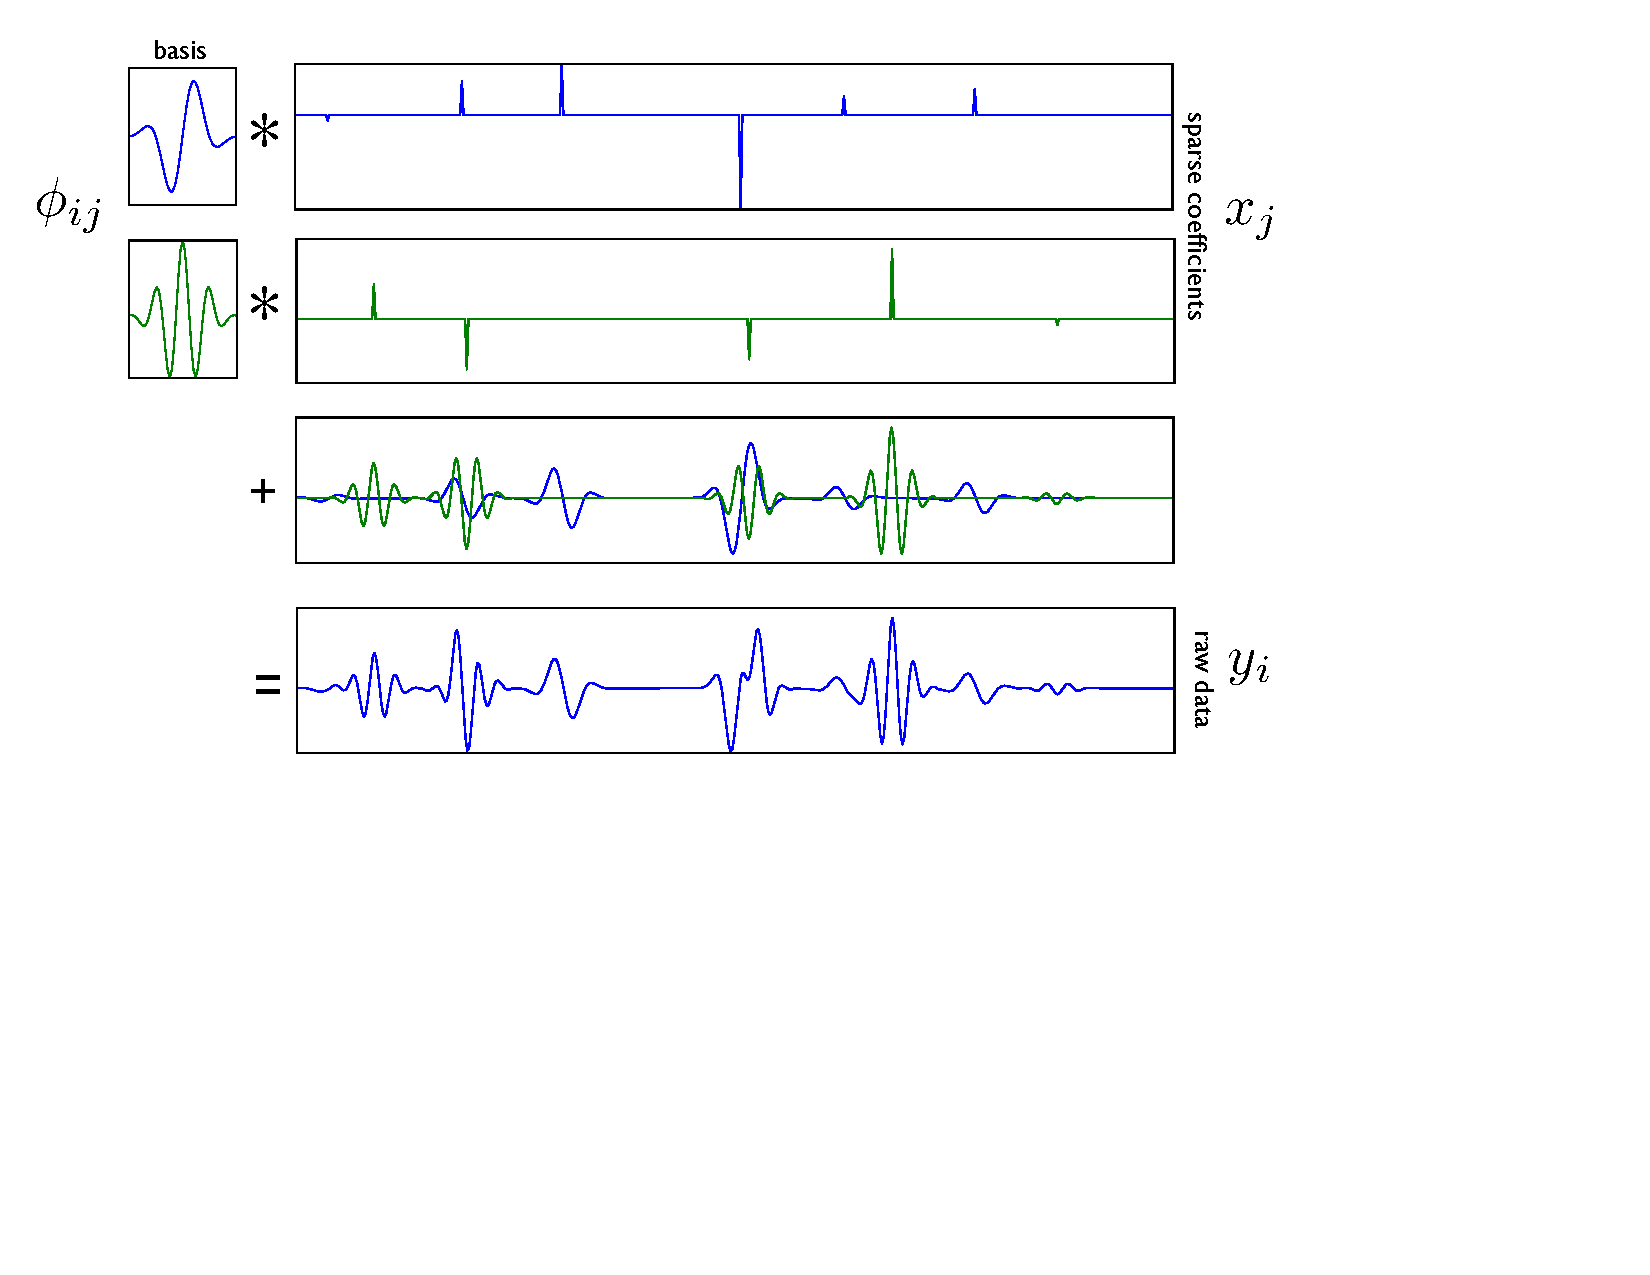
\includegraphics[width=0.9\textwidth]{fig1.pdf}
  \caption{\textbf{Convolutional sparse coding.} A convolutional
    sparse coding model is a linear generative model where data is
    represented as a sum of a convolution of a set of bases with
    coefficients which are expected to be sparse and independent in
    both time and channel. This schematic shows how to reconstruct a
    portion of one channel of data at bottom using two basis elements
    at left convolved with corresponding sparse coefficients at right
    and summed. Estimation of basis functions $\phi_{ij}$ and
    coefficients $x_j$ (Eq.~\ref{eqn:conv}) are called
    `learning' and `inference', respectively. Bases $\phi_{ij}$ are
    learned for spiking and LFP datasets separately for each recording
    penetration and coefficients are inferred for the entire
    recordings. This new representation has many desirable
    properties.}
  \label{fig:sparseconvolution}
\end{figure}

\subsection{Matching pursuit inference}

The nature of the spiking and LFP datasets required the inference
problem~\ref{eqn:inference} to be solved the using a different
strategy for each case. For the spike dataset, which is made up
primarily of highly sparse spike activity separated in time as well as
in space among the channels and mixed with approximately gaussian
noise, a greedy algorithm, matching
pursuit~\cite{mallat1993matching,olshausen2003learning,Smith:2006qf},
was chosen. This algorithm is efficient for a high degree of assumed
sparsity when the basis functions can be assumed to be relatively
incoherent. Its goal is to represent the data with at most $k$ basis
functions,
\begin{align*}
  \mb{x}^* = \argmin_{\card{\mb{x}} \le k} \frac{1}{2 \sigma_n^2}
  \sum_{t=1}^T \norm{\mb{y}_t - \sum_\tau \mb{\Phi}_\tau
    \mb{x}_{t-\tau}}^2
\end{align*}
where $\card{\mb{x}}$ denotes the number of non-zero elements of
$\mb{x}$. For arbitrary $\mb{\Phi}$, this problem is
NP-hard\cite{davis1997adaptive}. Matching pursuit is a greedy strategy
that finds an approximate solution and overcomes this combinatorial
complexity. Additionally, to make the learned basis functions and
coefficients more physiologically interpretable, the coefficients were
forced to be non-negative.

\subsection{L$_1$-regularized quasi-Newton inference}
\label{sec:quasinewton}

For the LFP dataset, an L$_1$-regularized method was used to induce
sparsity on the coefficients. The LFP dataset is sampled at a lower
rate and is hence considerably smaller than the spike dataset,
reducing requirements for computational efficiency by a large
factor. An L$_1$ method performed better at learning in a less sparse
regime where basis functions were more coherent and `explaining away'
was more critical. Briefly, the prior on coefficients was assumed to be
exponentially distributed,
\begin{align*}
  p(\mb{x}|\lambda) \propto e^{-\lambda \norm{\mb{x}}_1}
\end{align*}
giving the following convex minimization problem for inference,
\begin{align*}
  \mb{x}^* = \argmin_{\mb{x}>0} \frac{1}{2 \sigma_n^2} \sum_{t=1}^T
  \norm{\mb{y}_t - \sum_\tau \mb{\Phi}_\tau \mb{x}_{t-\tau}}^2_2 +
  \lambda\norm{\mb{x}}_1
\end{align*}
This objective is closely related to the Lasso, which has been
intensively studied~\cite{tibshirani1996regression,chen1999atomic} and
for which an abundance of methods exist. Despite its widespread use as
a feature selection method, it is important to note that an L$_1$
regularizer has a deficiency. If the data is indeed generated by a
Laplacian distribution, its order statistics are not sufficiently
sparse to guarantee recovery~\cite{baraniuk2010low}. Additionally,
both inference methods used are not causal, and coefficients inferred
for a given time can be affected by data in the future. In contrast,
state-space models such as Kalman filters and hidden Markov models are
causal by design, though operations such as smoothing are inherently
acausal. Creating a causal inference algorithm in this setting is an
open problem that is the subject of future work.

\section{Implementation}

For convolutional matching pursuit, the algorithm was implemented in
\texttt{python} using the \texttt{numpy}~\cite{numpyscipy}
library. For L$_1$-regularized inference, a
method~\cite{andrew2007scalable} based on the widely used l-BFGS
quasi-Newton algorithm~\cite{Liu89} was chosen, which uses a
particular choice of sub-gradient whenever the optimization attempts
to cross from one octant to another. The advantages of this algorithm
over the many others is that it does not require computing the Gram
matrix, only requires an objective and gradient to be defined, is
numerically stable for large numbers of parameters, converges quickly
to an approximate solution, and can be efficiently run in parallel on
multiple cores of a processor as it uses only BLAS level 1 operations.

Three versions of this algorithm were implemented. The first was a
\texttt{cython}\cite{behnel2011cython,seljebotn2009fast} wrapper of
the \verb!C++! library \texttt{liblbfgs}~\cite{liblbfgs}, which
explicitly implements all linear algebra with SSE2 instructions. Next,
a version in \texttt{cython} was implemented that could handle a
vector of L$_1$ regularization parameters $\lambda$, a non-negative
constraint on the coefficients, and would run more efficiently on
multicore architectures through its use of vendor linear algebra
libraries. Lastly, a version in \texttt{cython} and
\texttt{pycuda}~\cite{pycuda} was implemented to run fully on the
NVIDA GPU avoiding all host to GPU transfers during the
optimization. In this implementation, the convolutions in the
objective were implemented both as a bank of 2-D FFTs as well as a
single 3-D FFT. The 3-D FFT method, despite its theoretical
inefficiency in this case, gave an approximately 30x speed-up versus
computing the convolutions in the time domain on the CPU. The 2-D FFT
bank gave only a 6x speed-up, most likely due to the GPU being
constrained to computing one 2-D FFT at a time. Array slicing was
implemented with 1-D texture maps and all norms, projections, and
reductions were custom written to take advantage of the parallelism in
the GPU.

The full learning algorithm was parallelized using the Message Passing
Interface (MPI) in \texttt{python} using
\texttt{mpi4py}~\cite{seljebotn2009fast}. On each learning iteration,
the root node sampled the data from disk and distributed this data
amongst the nodes using an MPI \texttt{Scatter}. All nodes then
performed inference using one of the algorithms described above and
the results were reduced on the root node with an MPI
\texttt{Gather}. A learning step was taken and the basis was then MPI
\texttt{Broadcast} to all nodes. This framework allowed the learning
algorithm to exploit parallelism on a single multicore CPU with or
without a GPU, a cluster of multicore CPU's, as well as a hybrid
cluster of CPU's and GPU's.

\subsection{Parallel inference of coefficients for a full dataset}
\label{sec:parallelblock}

After a basis was learned for a spike or LFP dataset, coefficients
were inferred for the whole dataset in a chunk-wise parallel fashion
(Fig.~\ref{fig:parallelblock}). Given $N$ parallel computational
nodes, the data was divided into $N$ large chunks. Within each chunk,
inference was performed in sequence on blocks of time length $T$ with
$T >> P$, where $P$ is the number of time taps in the learned basis
$\mb{\Phi}$. Blocking was used at it is computationally impractical to
perform inference on arbitrarily large time segments. A block of
length $T$ yielded coefficients $\mb{x}$ of time length $T+P-1$. After
one block was completed, all except a $P-1$ length of its tail was
written to disk. The $2P-2$ tail portion of this block was used for
initializing the next block. For the new block, the first $P-1$
coefficients were held fixed whereas the next $P-1$ coefficients were
used to warm start the inference in the case of L$_1$ or were set to
zero for matching pursuit.

\begin{figure}[ht!]
  \centering
  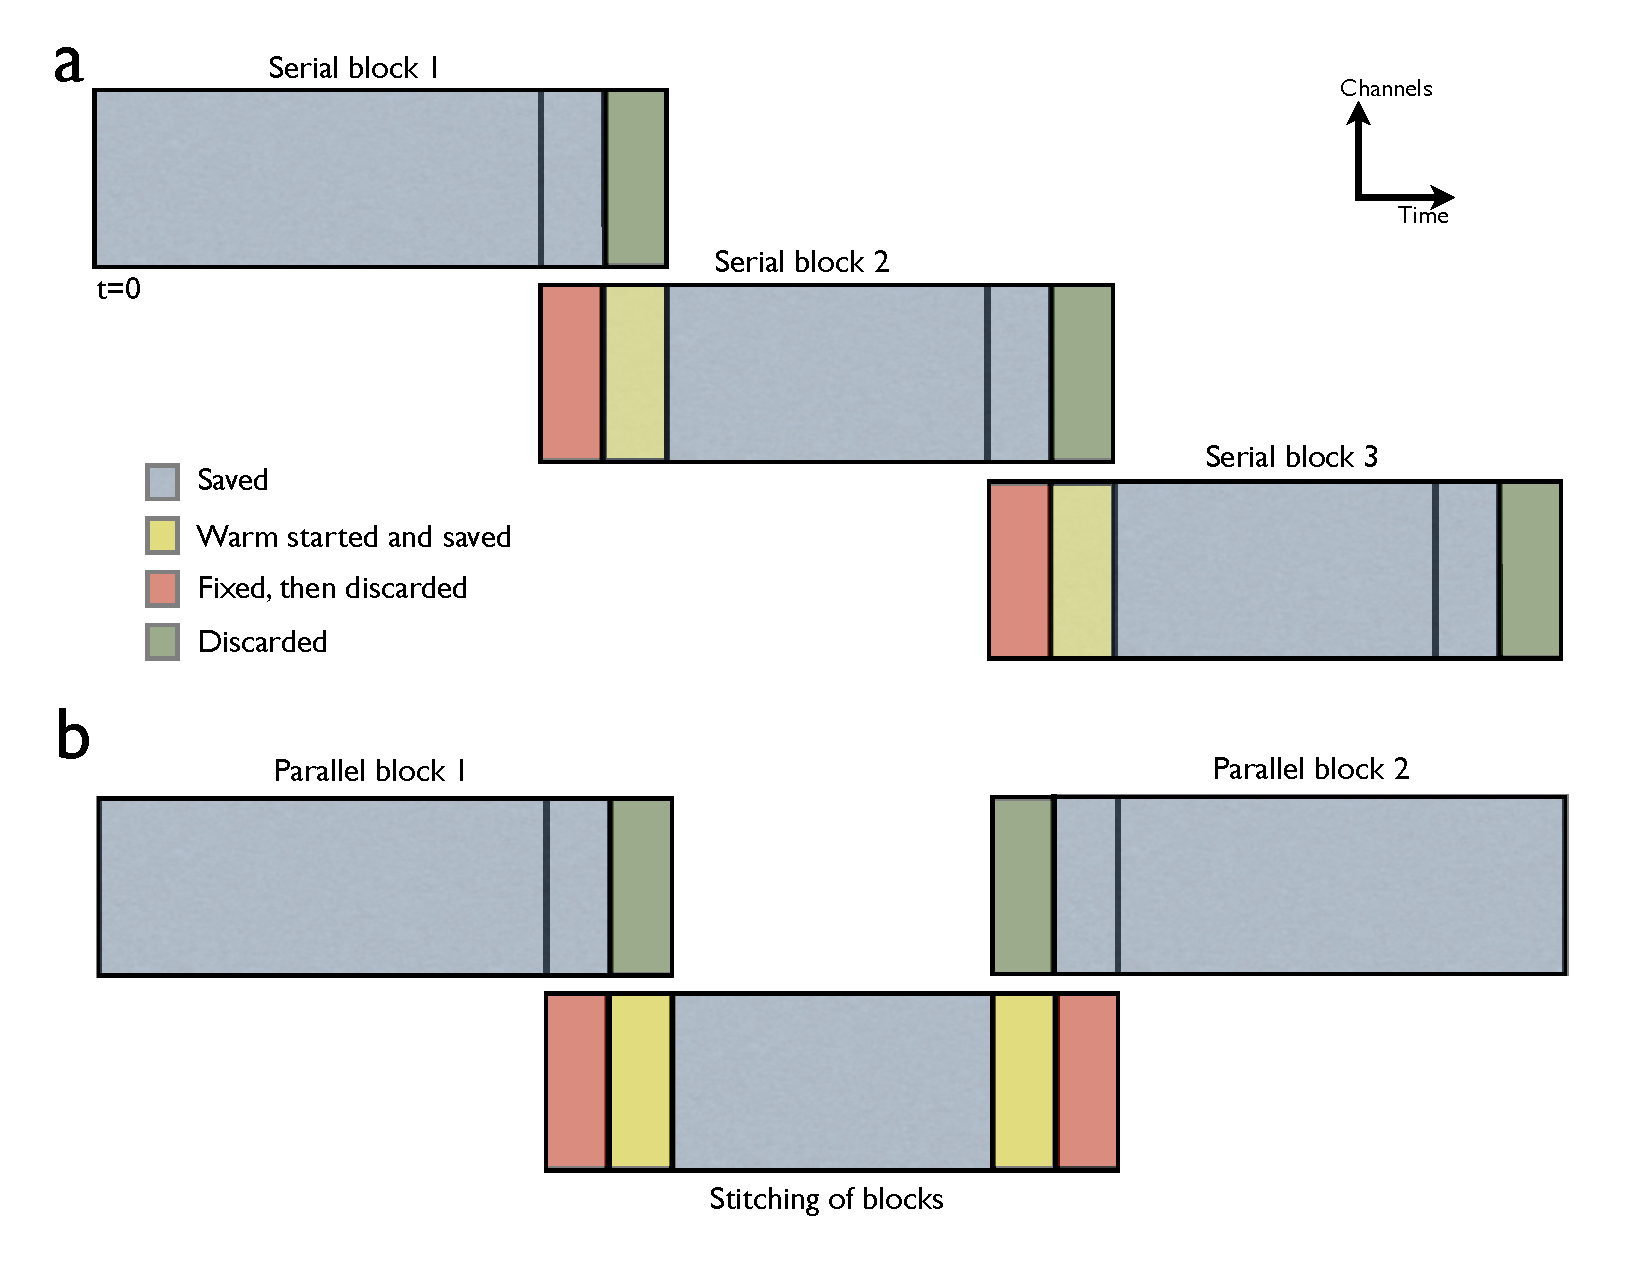
\includegraphics[width=0.9\textwidth]{fig6.pdf}
  \caption{\textbf{Inferring coefficients over a full dataset.}
    \textbf{(a)} Each parallel chunk of data is blocked into tractable
    portions and processed serially by using tail portions of previous
    blocks to warm-start the following block. \textbf{(b)} When each
    parallel chunk is completed, the regions between chunks are
    processed to stitch chunks into one long set of coefficients. The
    stitched portion is warm-started from it's adjoining blocks.}
  \label{fig:parallelblock}
\end{figure}

The non-linear nature of inference raised the possibility that the
implementation would have blocking artifacts. However, inference was
tested by blocking over a several block region as well as inferring
coefficients on the whole region with results in good agreement. This
is due to the high degree of sparsity used as well as a side-effect of
the convolutional formulation of the objective, that coefficients on
the $P-1$ borders received less derivative information and were more
likely to remain at zero.

Parallel blocks were stitched by performing inference on adjoining
regions of length $3P-2$, with only the inner $P-2$ portion being free
to be modified by the optimization. The parallel blocking allowed the
inference to scale almost linearly and to compute coefficients for a
recording session with approximately the same order of time as the
experiment itself. The datasets with metadata were written to disk
using a generic gzip level 4 compressed HDF5 format which afforded a
20-100 fold compression over the original dataset, depending primarily
on the level of coefficient sparsity.


\end{document}